%% ****** Start of file aiptemplate.tex ****** %
%%
%%   This file is part of the files in the distribution of AIP substyles for REVTeX4.
%%   Version 4.1 of 9 October 2009.
%%
%
% This is a template for producing documents for use with 
% the REVTEX 4.1 document class and the AIP substyles.
% 
% Copy this file to another name and then work on that file.
% That way, you always have this original template file to use.

\documentclass[aip,reprint]{revtex4-1}
%\documentclass[preprint]{revtex4-1}

\usepackage{xr-hyper}
\usepackage{array}
\usepackage{comment}

\makeatletter

\newcommand*{\addFileDependency}[1]{
\typeout{(#1)}
\@addtofilelist{#1}
\IfFileExists{#1}{}{\typeout{No file #1.}}
}\makeatother

\newcommand*{\myexternaldocument}[1]{%
\externaldocument{#1}%
\addFileDependency{#1.tex}%
\addFileDependency{#1.aux}%
}

\usepackage{hyperref}
\hypersetup{
    colorlinks=true,
    linkcolor=blue,
    filecolor=magenta,      
    urlcolor=cyan,
    pdftitle={Overleaf Example},
    pdfpagemode=FullScreen,
    }

\externaldocument[supp-]{si}
\myexternaldocument{si}

\usepackage{graphicx}% Include figure files
\usepackage{dcolumn}% Align table columns on decimal point
\usepackage{bm}% bold math
\usepackage{amssymb}
\usepackage{comment}
\usepackage{xcolor}
\usepackage{amsmath}

\usepackage[utf8]{inputenc}
\usepackage[T1]{fontenc}
\usepackage{mathptmx}
\usepackage{etoolbox}
\usepackage{verbatim}
\usepackage{lineno}
%\linenumbers

%\preprint{AIP/123-QED}
%\draft % marks overfull lines with a black rule on the right

\begin{document}

% Use the \preprint command to place your local institutional report number 
% on the title page in preprint mode.
% Multiple \preprint commands are allowed.
\preprint{}

\title{Template for Computational Physics Report}

\author{Candidate ID number}

\begin{abstract} 
\section*{Abstract}
\textbf{The abstract gives the reader a quick overview of what has been done and the most important results. Here is a typical example taken from a scientific article:}
\\
Heat conduction in calcium carbonate (CaCO$_3$) is of significant interest due to its wide applications in geological processes, biominerals, and industrial materials. This computational project investigates the thermal conductivity of calcium carbonate by solving the heat conduction equation using numerical integration techniques. Gaussian Quadrature is employed to evaluate integral terms in the steady-state heat conduction equation for homogeneous CaCO$_3$ samples, while Monte Carlo (MC) methods are applied to model stochastic heat transport in heterogeneous or polycrystalline structures. The study explores the effects of temperature gradients, crystal orientation, and microstructural variations on heat flux and effective thermal conductivity. Simulations are validated using experimental data for pure calcite and aragonite phases, demonstrating good agreement with known thermal properties. The results provide insights into the influence of microstructural anisotropy and impurities on heat conduction in CaCO$_3$, offering a computational framework for optimizing its use in energy storage, cement production, and geological modeling.
\end{abstract}

\maketitle 


\section{Introduction}

\textbf{The introduction should focus on the following aspects:}
\begin{enumerate}
    \item In the first part give a motivation for the work and overarching ideas.
    \item Give a scientific background of the topic and explain the rationale behind the project.
    \item Explain what you have done.
    \item Give the structure of the report and its organization.
\end{enumerate}
Example:
\begin{enumerate}
    \item Calcium carbonate is one of the most abundant minerals on Earth.\cite{deer2013introduction} It is involved in a variety of natural processes, such as the carbon dioxide sequestration process via aqueous wollastonite carbonation, \cite{Wouter_wollastonite, CO2_seqestation} and the biomineralization of exoskeletons and shells of marine organisms in water.\cite{Biomin_mollusc} ...
    \item The heat conduction in calcium carbonate has been previously studied by numerous experimental and modeling works. \cite{Bayarjargal_phase_diagr_VII} 
    \item In this work, I investigated ...
    \item The paper consists of an Introduction, a Models and Methods Section, and a Results and Discussion Section. In Section ...
\end{enumerate}

\section{Models and Methods}\label{sec:method}
\textbf{The methods section is very important in this computational project. It should focus on:}
\begin{enumerate}
    \item Describe the methods and algorithms you have chosen to treat the topic. Justify your choice and mention the stability and accuracy of the methods.
    \item Explain how you have implemented those methods.
    \item Possibly, discuss how your codes can reproduce benchmark or previous results that could be numerical and/or closed-form expressions.
\end{enumerate}

Examples: 

I have used the quadrature methods to evaluate integral terms in the steady-state heat conduction equation for homogeneous CaCO$_3$ samples and the Monte Carlo (MC) methods are applied to model stochastic heat transport in heterogeneous or polycrystalline structures.

The heat equation is...

The heat transport can be modeled considering... 

There are several quadrature methods. 

\subsection{Newton-Cotes Quadrature methods}\label{sec:methodGQ}
\begin{figure}[h!]
    \centering
    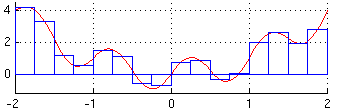
\includegraphics[width=1\linewidth]{figures/GAUSSIANQ.png}
    \caption{Illustration of the rectangle rule. The picture has been extracted from \href{https://en.wikipedia.org/wiki/Numerical_integration}{Wikipedia}.}
    \label{fig:enter-label}
\end{figure}

I implemented the high-order Newton-Cotes formulas in python using the following Algorithm Framework:

\begin{figure}[h!]
    \centering
    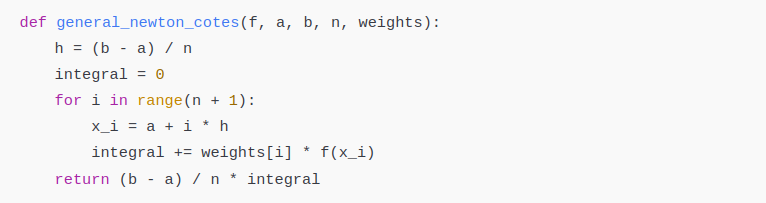
\includegraphics[width=1\linewidth]{figures/NewtonCotesAlgorithm.png}
    \caption{code snippet to showcase how I implemented the Newton-Cotes algorithm with Python.}
    \label{}
\end{figure}
where... 

However, the Newton-Cotes methods have stability and accuracy limitations that can arise from several factors, including oscillatory behavior, round-off errors, and numerical instabilities in certain situations...

\subsection{Gaussian Quadrature}\label{sec:methodGQ}
Gaussian Quadrature methods are advanced numerical integration techniques that provide highly accurate approximations of definite integrals by choosing optimal evaluation points (nodes) and weights according to the following formula:

\begin{equation}[h] 
\int _a^b f(x) dx \approx \sum _{i=1}^n w_i f(x_i) \\
\label{}
\end{equation}

where $x_i$ are nodes and $w_i$ corresponding weights. 

Gaussian Quadrature methods are highly efficient and accurate, but they can face certain limitations related to stability and accuracy, depending on the context in which they are applied...

\subsubsection{Gaussian-Legendre}
The Gaussian-Legendre variant approximates the nodes using the roots of the $n$-th Legendre polynomials $P_n(x)$ and calculates the weights $w_i$ using the derivatives of the Legendre polynomials. 
 
I implemented the calculation of the polynomial...

\subsubsection{Gaussian-Laguerre}
The Gaussian-Laguerre variant approximates the nodes using the roots of the $n$-th Laguerre polynomials $L_n(x)$ and calculates the weights $w_i$ using the $n-1$-th Laguerre polynomial. 

I implemented them...

Comparison between Gaussian and trapezoidal numerical integration techniques are shown in Fig.\ref{fig: CompaNC_GQ} of Appendix \ref{A1}. 

\subsection{Monte Carlo Integration}\label{sec:methodMC}

Monte Carlo (MC) Integration is a numerical method that estimates the value of an integral using random sampling. It is especially useful for high-dimensional or complex integrals where traditional methods like Gaussian Quadrature are inefficient.

In Fig. \ref{fig:MC} the results from the Numerical integration by MC to calculate $\pi$ are shown. 
 

\begin{figure}[h!]
    \centering
    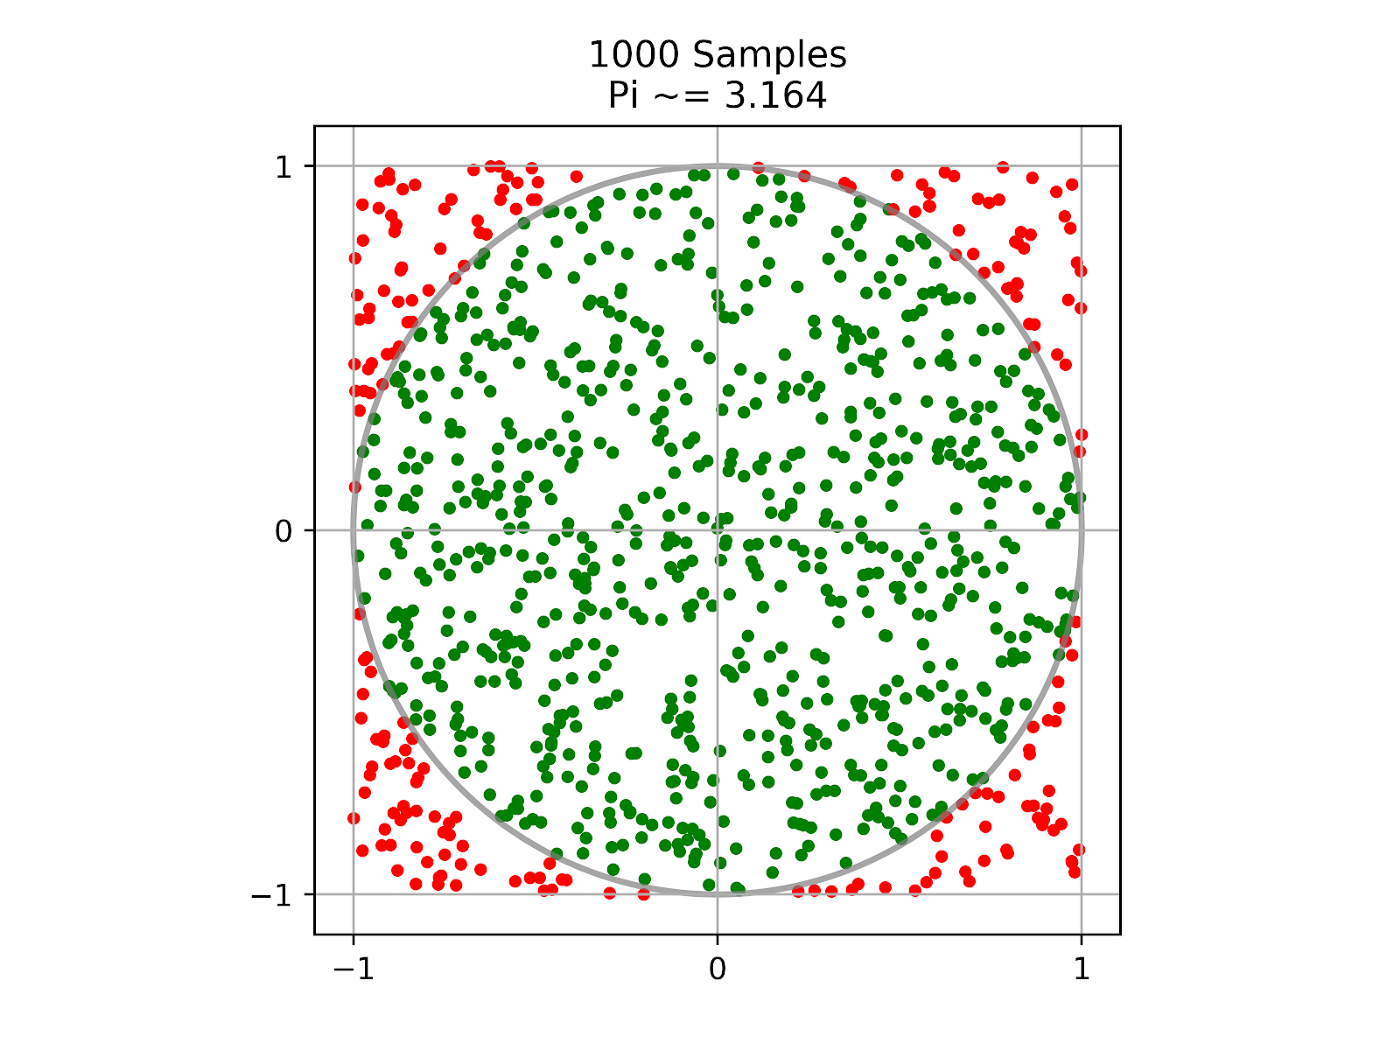
\includegraphics[width=0.6\textwidth]{figures/monte_carlo_pi.png}\\
    \caption{Monte Carlo integration methods to calculate $\pi$ by using the number of random samples that lie in the unit circle $\pi$. The picture have been extracted from \href{https://en.wikipedia.org/wiki/Gaussian_quadrature}{Wikipedia}.}  
    \label{fig:MC}
\end{figure}

\subsubsection{Brute force: uniform distribution}

\subsubsection{Importance sampling}

The advantages of using MC integration are...

However, the accuracy depends on...

\section{Results and Discussion}\label{sec:results}

We divide this Section into two parts, considering first the results I have obtained using the Gaussian Quadrature methods explained in Section \ref{sec:methodGQ}, the numerical integration and by Monte Carlo methods in Section \ref{sec:methodMC}. 

\subsection{Numerical Integration results by Gaussian Quadrature}
\subsubsection{Gauss-Legendre}

\begin{table}[h] % [h] forces the table to appear "here" in the document
    \centering % Centers the table on the page
    \caption{Your table caption here} % Adds a caption
    \label{tab:my_table} % Adds a label for cross-referencing
    \begin{tabular}{|c|l|r|} % Defines three columns: centered, left-aligned, right-aligned, all with vertical lines
        \hline % Horizontal line
        \textbf{Header 1} & \textbf{Header 2} & \textbf{Header 3} \\ % Column headers with cell separation using & and row end with \\
        \hline % Horizontal line
        Row 1, Cell 1 & Row 1, Cell 2 & Row 1, Cell 3 \\
        Row 2, Cell 1 & Row 2, Cell 2 & Row 2, Cell 3 \\
        \hline % Horizontal line
    \end{tabular}
\end{table}

\subsubsection{Gauss-Laguerre}

 

\subsection{Numerical Integration by Monte Carlo methods}\label{subsec:temp}

\subsubsection{Brute force Monte Carlo}


Brute force Monte Carlo is a straightforward, flexible approach for numerical integration, especially useful for high-dimensional or complex problems. The approximations using this technique become fairly good. However, its slow convergence means it may not be the most efficient for simple problems with low dimensions or smooth integrands.

\subsubsection{importance sampling}

The results using importance sampling are even better. 
While brute force Monte Carlo is a simple and general approach, importance sampling offers a powerful way to reduce variance and improve convergence for complex integrals. Importance sampling is often preferred in cases where the integrand is difficult to sample from uniformly, but it requires more careful setup and a good proposal distribution.


Fig.~\ref{fig: Good} of Appendix \ref{B1} shows the integral calculations by MC techniques.

\section{Conclusions}\label{sec:conclusions}

\textbf{The conclusions section should focus on:}
\begin{enumerate}
    \item Stating the main findings and interpretations of those.
    \item Giving as much as you can a perspective for further work on the same topic. 
    \item Discussing advantages and disadvantages of the methods used, possible improvements and/or alternatives.
\end{enumerate}



Example: 

In this project, I have studied heat conduction in calcium carbonate (CaCO$_3$) by solving the heat conduction equation using numerical integration techniques. The study explores the effects of temperature gradients, crystal orientation, and microstructural variations on heat flux and effective thermal conductivity. Simulations are validated using experimental data for pure calcite and aragonite phases, demonstrating good agreement with known thermal properties. The results provide insights into the influence of microstructural anisotropy and impurities on heat conduction in CaCO$_3$, offering a computational framework for optimizing its use in energy storage, cement production, and geological modeling.

Additional work can be done to verify...

\section*{REFERENCES}
\textbf{This part should contain all the references you have used.}

\begin{itemize}
    \item Give always references to material you have used to perform your work, books, journal articles, reports, and electronic resources.
    \item The articles’ references should present at least: the name(s) of author(s), journal, volume (boldfaced), page, and year in parenthesis.
    \item The books’ references should present at least: the name(s) of author(s), title of book, publisher, place and year, and eventual page numbers.
 
\end{itemize}


\bibliography{articles}

\newpage
\section*{Appendix A: Gaussian quadrature}
While brute force Monte Carlo is a simple and general approach, importance sampling offers a powerful way to reduce variance and improve convergence for complex integrals. Importance sampling is often preferred in cases where the integrand is difficult to sample from uniformly, but it requires more careful setup and a good proposal distribution.

\begin{figure}[h!]
    \centering
    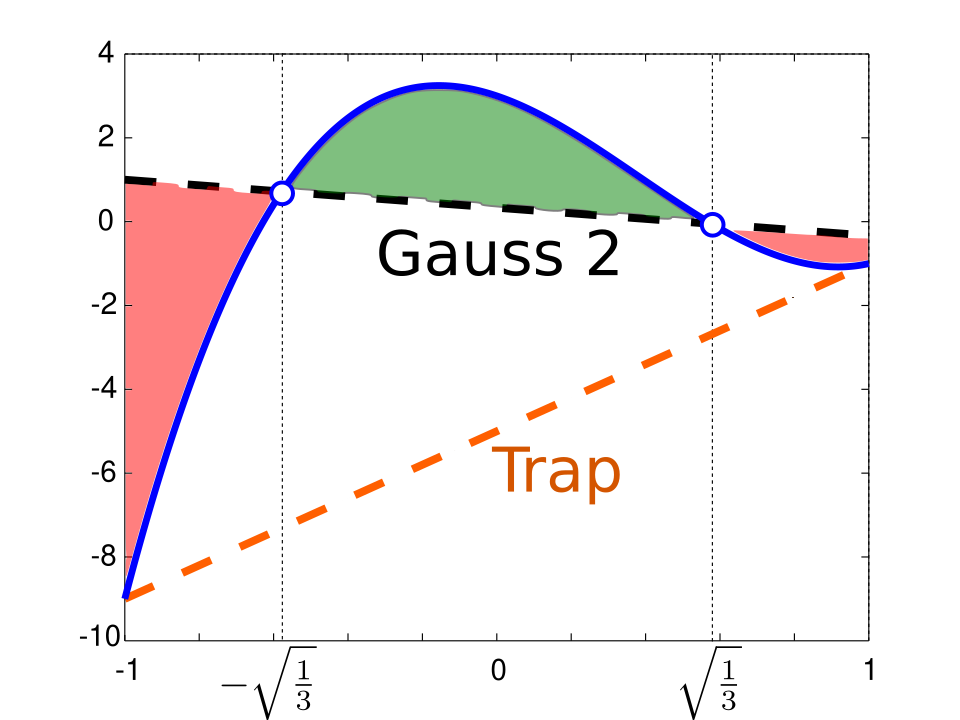
\includegraphics[width=0.8\linewidth]{figures/Comparison_Gaussquad_trapezoidal.svg.png}
    \caption{Comparison between Gaussian and trapezoidal numerical integration techniques. The 2-point rule gives you an exact result because the area of the lighter grey regions equals the area of the dark grey region.}
    \label{fig: CompaNC_GQ}
\end{figure}

\section*{Appendix B: Monte Carlo}

The Monte Carlo rejection method is a simple technique used to sample from a probability distribution when direct sampling is difficult. It is a widely used method in numerical simulations and computational physics. Below is an explanatory sketch of the method.

\begin{figure}[h]
    \centering
    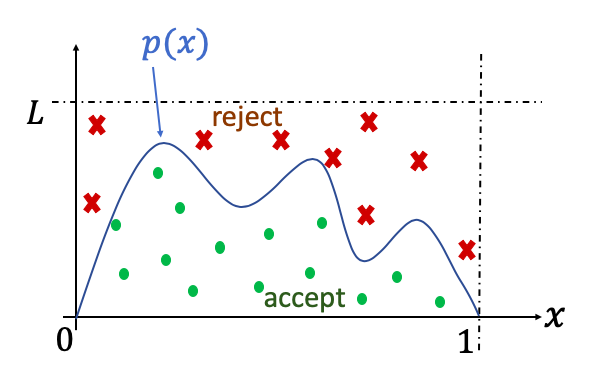
\includegraphics[width=0.96\linewidth]{figures/MCintegration.png}
    \caption{Monte Carlo rejection method}
    \label{fig: Good}
\end{figure}

\end{document}
%
% ****** End of file aiptemplate.tex ******